%This is a Latex file.
\documentclass[12pt]{article}
\usepackage{latexsym,fancyhdr,amsmath,amsfonts,amsthm,dsfont}
\usepackage{amssymb}
\usepackage{tikz}
\usetikzlibrary{calc}

% margins are relative to the default of 1 in
%\topmargin       -0.2 in

\topmargin        -0.2 in
\textheight       8.4 in
\oddsidemargin    0 in     % this is for pages 1, 3, 5, ...
\evensidemargin   0 in     % and this for 2, 4, 6, ...
\textwidth        6.5 in
%\headheight       15 in     % we won't have a running head, nor
\headsep          .35 in     % any extra space between head and text

%\parindent 0pt

\pagestyle{fancy} \lhead{\sf MTH 317} \chead{\sf Homework 2}
\rhead{\sf Rayana Gottschall} \lfoot{} \cfoot{} \rfoot{}

\newcommand{\C}{\mathds{C}}
\newcommand{\I}{\mathds{I}}
\newcommand{\N}{\mathds{N}}
\newcommand{\Q}{\mathds{Q}}
\newcommand{\R}{\mathds{R}}
\newcommand{\Z}{\mathds{Z}}

\begin{document}
\begin{enumerate}
\item[1.22] Let $G$ be a disconnected graph. By Theorem 1.11, $\overline{G}$ is connected. 
    Prove that if $u$ and $v$ are any two vertices of $\overline{G}$, then $\operatorname{diam}(\overline{G}) \leq 2$.
\begin{proof}
Let $G$ be a disconnected graph with vertex set $V$ and let $\overline{G}$ be its complement.
We show that for any $u,v\in V$ the distance $d_{\overline{G}}(u,v)\le 2$, whence $\operatorname{diam}(\overline{G})\le 2$.

If $u=v$ then $d_{\overline{G}}(u,v)=0\le2$, so assume $u\neq v$.

There are two cases.

\emph{Case 1: $u$ and $v$ lie in different connected components of $G$.}  
Then $u$ and $v$ are not adjacent in $G$, so the edge $uv$ belongs to $\overline{G}$. Hence
$d_{\overline{G}}(u,v)=1\le2$.

\emph{Case 2: $u$ and $v$ lie in the same connected component of $G$.}  
Since $G$ is disconnected, there exists a vertex $w\in V$ that lies in a component different from the component containing $u$ (and thus different from the component containing $v$). Therefore neither $uw$ nor $vw$ is an edge of $G$, so both $uw$ and $vw$ are edges of $\overline{G}$. Thus there is a path $u-w-v$ of length $2$ in $\overline{G}$, so $d_{\overline{G}}(u,v)\le 2$.

In every possible case we have $d_{\overline{G}}(u,v)\le 2$. Since $u$ and $v$ were arbitrary vertices of $\overline{G}$, it follows that $\operatorname{diam}(\overline{G})\le 2$.
\end{proof}

    
\item[1.24] Determine whether the graphs $G_1$ and $G_2$ are bipartite. If a graph is bipartite, then redraw it indicating the 
    partite sets; if not, then give an explanation as to why the graph is not bipartite.
\item[1. ]
    \begin{center}
    G\textsubscript{1} is bipartite.  
    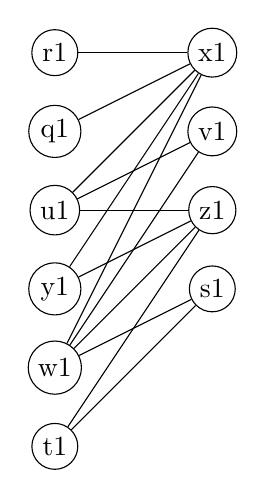
\begin{tikzpicture}[scale=1, every node/.style={circle, draw, fill=white, inner sep=2pt}]
    \node (r1) at (0,5) {r1};
    \node (q1) at (0,4) {q1};
    \node (u1) at (0,3) {u1};
    \node (y1) at (0,2) {y1};
    \node (w1) at (0,1) {w1};
    \node (t1) at (0,0) {t1};
    \node (x1) at (2,5) {x1};
    \node (v1) at (2,4) {v1};
    \node (z1) at (2,3) {z1};
    \node (s1) at (2,2) {s1};

    \draw (r1) -- (x1);
    \draw (q1) -- (x1);
    \draw (u1) -- (x1);
    \draw (u1) -- (v1);
    \draw (u1) -- (z1);
    \draw (y1) -- (x1);
    \draw (y1) -- (z1);
    \draw (w1) -- (x1);
    \draw (w1) -- (v1);
    \draw (w1) -- (z1);
    \draw (w1) -- (s1);
    \draw (t1) -- (z1);
    \draw (t1) -- (s1);
    \end{tikzpicture}
    \end{center}
\item[2.]
\begin{center}
    $G_2$ is not bipartite because it contains at least one odd cycle of order 5. 
\end{center}

\item[1.33] A diagraph D has vertex set {-3, 3, 6, 12} and ${i, j} \in D$ 
if $i \neq j$ and j is a multiple of i.
\begin{center}
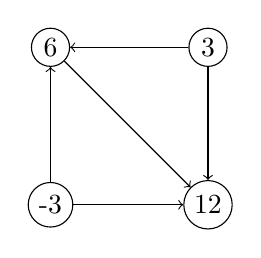
\begin{tikzpicture}[scale=1, every node/.style={circle, draw, fill=white, inner sep=2pt}]
    \node (n3a) at (0,0) {-3};
    \node (n3b) at (2,2) {3};
    \node (n6) at (0,2) {6};
    \node (n12) at (2,0) {12};

    \draw[->] (n3a) -- (n6);
    \draw[->] (n3a) -- (n12);
    \draw[->] (n3b) -- (n6);
    \draw[->] (n3b) -- (n12);
    \draw[->] (n6) -- (n12);
\end{tikzpicture}
\end{center}
 
\item[2.4] Give an example of a Graph $G$ of order 6 and size 10 such that $\partial$(G) = 3 and $\Delta$(G) = 4.
\begin{center}
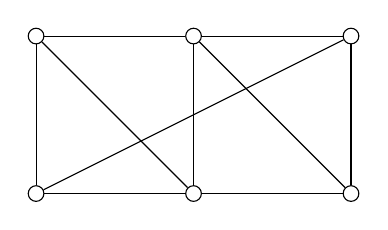
\begin{tikzpicture}[scale=1, every node/.style={circle, draw, fill=white, inner sep=2pt}]
    \node (A) at (0,0) {};
    \node (B) at (2,0) {};
    \node (C) at (2,2) {};
    \node (D) at (0,2) {};
    \node (E) at (4,2) {};
    \node (F) at (4,0) {};

    \draw (A) -- (B);
    \draw (A) -- (D);
    \draw (A) -- (E);
    \draw (B) -- (C);
    \draw (B) -- (D);
    \draw (B) -- (F);
    \draw (C) -- (D);
    \draw (C) -- (E);
    \draw (C) -- (F);
    \draw (F) -- (E);
\end{tikzpicture}
\end{center}
 
\item[2.6] Prove that if a graph of order 3$n$ ($n$ $\geq$ 1) has $n$ vertices of each of the degrees
\item[] $n$ - 1, $n$, and $n$ +1, then $n$ is even.
   \begin{proof}
Let $G$ be a graph of order $3n$ with $n$ vertices of each of the degrees $n-1$, $n$, and $n+1$.
By Theorem 2.1, the sum of degrees of a graph is 2$m$, where $m$ is the size of $G$. 2$m$ is even, so 3$n^2$ must be even. 
Since 3 is odd, $n^2$ must be even, and thus $n$ is even.
   \end{proof}
\end{enumerate}
\end{document}
